\chapter{Внедрение беспилотного транспорта и проблемы его применения} \label{chapt2}

\section{Необходимость применения беспилотного транспорта} \label{sect_Need}

Дорожные происшествия являются самой опасной
угрозой здоровью людей во всем мире. Ущерб от ДТП превышает
ущерб от всех иных транспортных происшествий (само­летов,
кораблей, поездов, и т. п.) вместе взятых. До­рожно-­транспортные
происшествия являются одной из
важнейших мировых угроз здоровью и жизни людей.
Проблема усугубляется и тем, что пострадавшие в ава­риях — как правило, 
молодые и здоровые (до аварии)
люди. По данным ВОЗ, в мире ежегодно в дорожных
авариях погибают 1,2 млн человек и около 50 млн по­лучают 
травмы. Более 27000 погибает на российских
дорогах, и более 40000 на дорогах США, в пересчете
на количество автомобилей эти цифры означают в год
70 погибших в ДТП на территории России или 15 по­гибших 
в США на каждые 100 000 автомобилей \cite{DTP_ukr}.
% Скопированно без изменений

Известно, что ДТП – непреднамеренное событие, возникающее в результате 
неблагоприятного сочетания факторов в
условиях динамической системы <<человек – автомобиль - дорога>>, вероятность 
которого может увеличиваться под
воздействием неблагоприятных внешних факторов (дождь, гололед, сумерки, дорожные 
работы, т.п.) и следствием
которого является ущерб здоровью человека, повреждение транспортного средства и 
дорожного обустройства.
Факторы, связанные с человеком, транспортным средством и дорожной 
инфраструктурой являются элементами единой
дорожно-транспортной системы, где множество элементов, находящихся в отношениях 
и связях друг с другом,
образуют определенную целостность. Изучение систем требует применения системного 
подхода. Системный подход
нацелен на выявление многообразных типов связей в системе и сведение их в единую 
теоретическую картину.
С точки зрения безопасности дорожного движения интерес для системного изучения 
представляют как сами факторы
риска, так и их различные сочетания, а именно:
\begin{itemize}
  \item человек/автомобиль;
  \item автомобиль/дорога;
  \item дорога/человек.
\end{itemize}

% Эта часть скопирована без изменений

Министерство транспорта Германии в 2002 г. провело исследования причин ДТП 
во многих странах мира. На рисунке \ref{img:dtp_roles} представлена примерная 
картина соотношения данных факторов \cite{DTP_factors}.
% Этот абзац изменен

\begin{figure}[ht] 
  \centering
  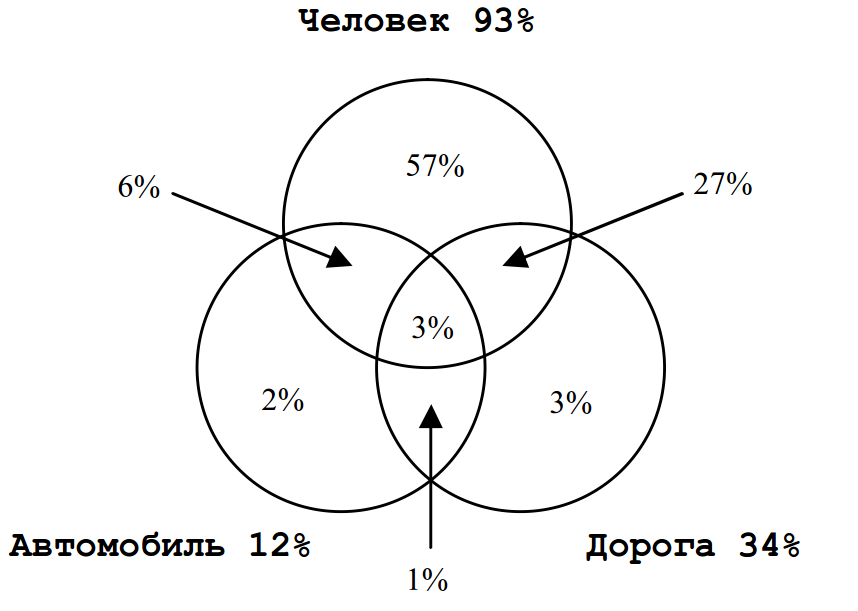
\includegraphics [scale=0.5] {dtp_roles}
  \caption{Роль факторов риска и их сочетаний в возникновении ДТП}
  \label{img:dtp_roles}
\end{figure}

По данной диаграмме можно сделать вывод, что:
\begin{itemize}
  \item главная причина ДТП в 57\% случаев – ошибка человека;
  \item еще в 6\% случаев - причиной является проблема взаимодействия человека и 
        автомобиля (например, интерференция навыков в критической ситуации);
  \item еще в 27\% случаев - причиной является проблема взаимодействия человека 
        и дороги (например, провоцирование водителя на превышение скорости 
        посредством прямого и широкого участка дороги за которым следует резкий 
        поворот);
  \item еще в 3\% случаев - причиной является проблема сложного взаимодействия 
        человека, автомобиля и дороги.
\end{itemize}

Таким образом в 93\% случаев ДТП присутствует человеческий фактор, который 
выражается следующими проявлениями:
\begin{enumerate}
  \item Превышение скорости;
    \begin{enumerate}
      \item недостаток опыта для выбора правильной скорости в
            определенных дорожных условиях (мокрое покрытие,
            гололед, снег, дождь,
      \item поведенческая ориентация,
    \end{enumerate}

  \item Игнорирование требований дорожных знаков;
    \begin{enumerate}
      \item непонимание причин установки дорожных знаков,
      \item частые случаи забытых знаков после производства дорожных
            работ или изменения условий движения,
      \item отсутствие баз данных по дислокации дорожных знаков,
      \item неправильная установка или плохое состояние дорожных
            знаков, что делает их малозаметными,
      \item перегрузка водителей информацией (неправильная
            установка рекламных щитов вместе с дорожными знаками),
    \end{enumerate}

  \item Игнорирование погодных и дорожных условий;
  \begin{enumerate}
    \item непонимание возможных последствий,
    \item переоценка собственных возможностей и/или возможностей автомобиля,
  \end{enumerate}

  \item Отсутствие уважения водителей по отношению к пешеходам;
    \begin{enumerate}
      \item низкая культура участников движения,
      \item недостаток контроля,
      \item наличие участков дорог, провоцирующих водителей на
            превышение скорости,
      \item неудобное размещение переходов для пешеходов,
      \item недостаток осознания риска дтп,
      \item незнание механизма торможения,
    \end{enumerate}

  \item Значительная доля молодых водителей (основная группа
        риска), как результат бурного роста автомобилизации;
    \begin{enumerate}
      \item курс подготовки водителей слишком краток, качество
            подготовки низкое,
      \item недостаток информации,
      \item поведенческая ориентация,
      \item недостаточность общественных кампаний, стимулирующих
            безопасный стиль вождения,
      \item отсутствие государственной политики в отношении
            продвижения правильных моделей поведения через сми
            (фильмы, реклама, литература, т.п.),
  \end{enumerate}

  \item Агрессивный стиль вождения, безопасная модель поведения
        среди российских водителей не популярна;
    \begin{enumerate}
      \item автомобиль рассматривается как средство демонстрации
            статуса и поднятия самооценки,
      \item недостаток информации,
  \end{enumerate}

  \item Игнорирование пассивных мер безопасности (шлемов, ремней
        безопасности, светоотражателей);
    \begin{enumerate}
      \item недостаток информации и осознания важности и
            необходимости мер безопасности,
      \item недостаток контроля,
  \end{enumerate}

  \item Управление транспортным средством в состоянии
        алкогольного опьянения;
    \begin{enumerate}
      \item недостаток информации и осознания риска,
      \item недостаток контроля,
      \item неэффективность законодательства,
      \item равнодушное отношение со стороны общественности.
  \end{enumerate}
\end{enumerate}

Также исследования показали, что водители, которые во
время езды слушают музыку, более склонны к пре­вышению скорости и чаще попадают 
в ДТП, так как становятся невнимательными \cite{DTP_Gladkiy}.
% Скопированно без изменений из DTP_ukr

Очевидно, что все проблемы, перечисленные выше можно решить, лишив человека 
необходимости управлять транспортным средством. По этим причинам развитие и внедрение 
беспилотного транспорта является не просто одним из направлений прогресса, а 
представляет собой необходимость с целью снижения смертности населения.

Согласно данным AT Kearney, беспилотный транспорт сокращает вероятность 
возникновения ДТП на 70\%. По
статистике число смертности и ДТП с участием автомобилей под управлением водителей
многократно превосходит показатели беспилотников \cite{Plus&Minus}.
% Скопированно без изменений из Plus&Minus

Современный мегаполис насчитывает большое количество машин, из-за чего огромные
пробки и заторы становятся главной проблемой в вопросе экономии времени. Беспилотный
автомобиль способен определять точные сведения о загруженности тех или иных улиц,
благодаря чему он с легкостью выберет оптимальный путь. Кроме этого город избавиться от
проблемы отсутствия парковочных мест за счет автономной системы парковки, которая
самостоятельно определит свободное парковочное место, и автомобиль займет его без
участия водителя. Все это приведет к повышению пропускной способности дорог 
\cite{Pilotless_Trust}.
% Скопированно без изменений из Plus&Minus

Беспилотный транспорт позволит снизить затраты на транспортировку грузов и
пассажиров. Во-первых, позволит экономить топливо. Если на трассе пять автомобилей
выстроятся в одну колонну, то пятая машина будет потреблять на 30\% меньше топлива, чем
первая. Допустим, фура весит 40 тонн. Чтобы преодолеть сопротивление ветра на скорости,
один автомобиль затратит больше топлива, чем колонна грузовиков, которые уже идут в
воздушном потоке. И если управление только первой машины будет осуществляться
водителем, а остальные будут беспилотными, то получим экономию на зарплатах и налогах.
Во-вторых, беспилотные автомобили уменьшают сроки доставки грузов более чем в 2
раза. Если обычная фура доезжает из Москвы в Екатеринбург за три дня, то с переходом на
беспилотное управление груз будет на месте уже через 35 часов. Водителю необходимо
время на сон и на отдых, что вызывает задержки в доставке груза. Несколько водителей
способны уменьшить время перевозки, но в свою очередь это увеличит финансовые 
затраты \cite{Pilotless_Future}.
% Скопированно без изменений из Plus&Minus

Для США были проведены количественные расчёты выгоды внедрения беспилотного 
транспорта \cite{Pilotless_Efimov}. Расчеты представлены в таблице 
\ref{tbl:economics_effect}. Как видно из таблицы при увеличении доли 
беспилотного транспорта, можно получить колоссальный экономический 
эффект.

\begin{table} [htbp]
  \caption{Экономический эффект внедрения беспилотного транспорта}
  \label{tbl:economics_effect}
  \begin{SingleSpace}
    \begin{tabular}{| l | l | l | l |}
      \hline
                                     & \multicolumn{3}{|c|}{Уровень проникновения} \\
      \multicolumn{1}{|c|}{Критерий} & \multicolumn{3}{|c|}{беспилотных транспортных средств} \\
      \cline{2-4}
      & \multicolumn{1}{|c|}{10\%} & \multicolumn{1}{|c|}{50\%} & \multicolumn{1}{|c|}{90\%} \\
      \hline
      \multicolumn{4}{|c|}{Экономический эффект от предотвращения ДТП} \\
      \hline
      Спасенные жизни (в год)       & 1 100        & 9 600         & 21 700        \\
      Предотвращение аварий         & 211 000      & 1 880 000     & 4 220 000     \\
      Снижение экономических затрат & \$5.5 млрд.  & \$48.8 млрд.  & \$109.7 млрд. \\
      Комплексное снижение затрат   & \$17.7 млрд. & \$158.1 млрд. & \$355.4 млрд. \\
      \hline
      \multicolumn{4}{|c|}{Уменьшение дорожных пробок} \\
      \hline
      Экономия времени (млн. часы.) & 756          & 1680          & 2772          \\
      Экономия топлива (млн. л.)    & 386          & 848           & 2740          \\
      Общая экономия                & \$16.8 млрд. & \$37.4 млрд.  & \$63.0 млрд.  \\
      \hline
      \multicolumn{4}{|c|}{Дополнительные преимущества} \\
      \hline
      Экономия на парковках         & \$3.2 млрд.  & \$15.9 млрд.  & \$28.7 млрд.  \\
      на одну машину                & \$250        & \$250         & \$250         \\
      \hline
      \multicolumn{4}{|c|}{Итого в год} \\
      \hline
      Экономический эффект          & \$25.5 млрд. & \$102.2 млрд. & \$201.4 млрд. \\
      Общий эффект                  & \$37.7 млрд. & \$211.5 млрд. & \$447.1 млрд. \\
      \hline
    \end{tabular}
  \end{SingleSpace}
\end{table}

Также в США был проведен опрос и исследование общественного мнения по 
поводу новшеств в автомобильной промышленности \cite{Social_AutoTech}. По
мнению большинства граждан США беспилотный транспорт принесет больше пользы
нежели вреда (рисунок \ref{img:social_advantages}).

\begin{figure}[ht] 
  \centering
  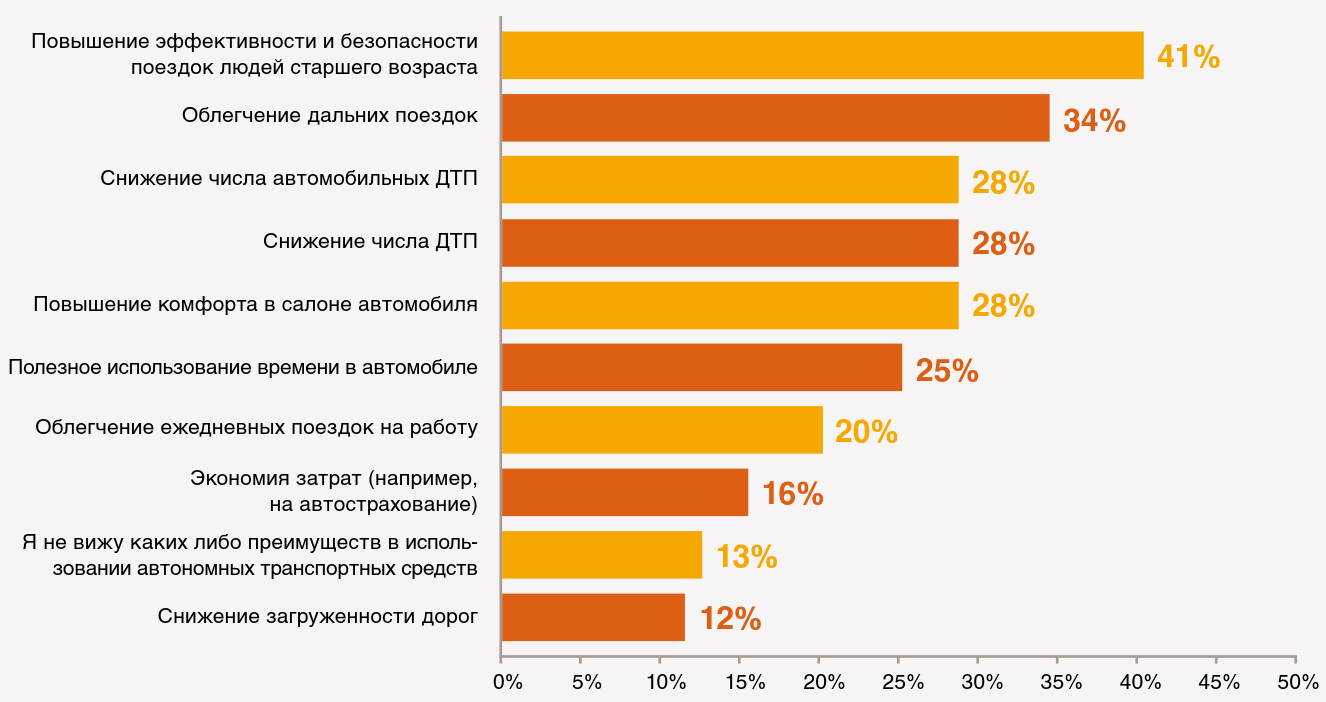
\includegraphics [scale=0.5] {social_advantages}
  \caption{Социальный опрос: преимущества автономных транспортных средств}
  \label{img:social_advantages}
\end{figure}

Описанные преимущества беспилотного транспорта громко заявляют о необходимости
его применения и развития. Чем скорее автопилот вытеснит человека, тем
скорее решатся многие проблемы транспорта, а также приблизится к решению одна
из глобальных проблем человечества -- экологическая.

%\newpage
%============================================================================================================================
\section{Безопасность беспилотного транспорта} \label{sect2_Security}

% Глава составлена из Pilotless_Integral и Pilotless_Tadviser с серезными
% правками с сокращениями

Несмотря на все преимущества беспилотного транспорта, его внедрение ограничивает
ряд проблем. Одна из основных -- это безопасность автопилота. В данном случае
очень важна моральная сторона вопроса. Первой на
пути решения этой проблемы встает классическая дилемма вагонетки:
неуправляемая вагонетка несется по 
рельсам. На основных путях привязаны пять человек, на запасных — еще один, а 
вы можете переключить железнодорожную стрелку и тем самым спасти пять жизней, 
взамен пожертвовав одной. С появлением БТС эта абстрактная этическая 
дилемма обретает плоть, поскольку создателям таких автомобилей надо раз и навсегда 
заложить в алгоритме, как будет действовать машина во всех спорных ситуациях
(рисунок \ref{img:ethical_cars}).

%%%%%%%% Моральная дилемма %%%%%%%%%
% http://www.tadviser.ru/index.php/%D0%A1%D1%82%D0%B0%D1%82%D1%8C%D1%8F:%D0%90%D0%B2%D1%82%D0%BE%D0%BF%D0%B8%D0%BB%D0%BE%D1%82_(%D0%B1%D0%B5%D1%81%D0%BF%D0%B8%D0%BB%D0%BE%D1%82%D0%BD%D1%8B%D0%B9_%D0%B0%D0%B2%D1%82%D0%BE%D0%BC%D0%BE%D0%B1%D0%B8%D0%BB%D1%8C)#.D0.9C.D0.BE.D1.80.D0.B0.D0.BB.D1.8C.D0.BD.D0.B0.D1.8F_.D0.B4.D0.B8.D0.BB.D0.B5.D0.BC.D0.BC.D0.B0
%%%%%%%%%%%%%%%%%%%%%%%%%%%%%%%%%%%%

\begin{figure}[ht] 
  \centering
  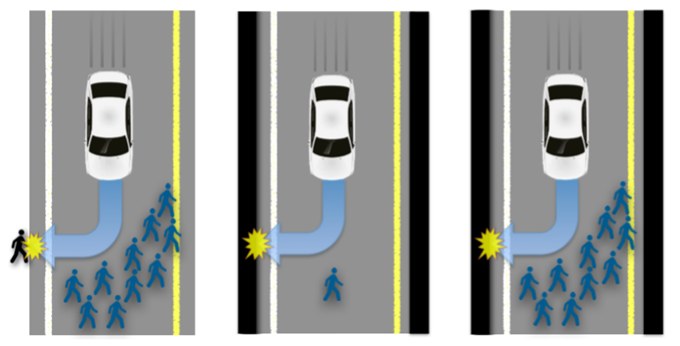
\includegraphics [scale=0.9] {ethical_cars}
  \caption{Сценарии для спорных решений беспилотного транспорта}
  \label{img:ethical_cars}
\end{figure}

Авторы исследования о социальной дилемме автономных автомобилей, 
опубликованного в журнале Science в 2016 году, полагают, что в это области 
есть и другие сложные моральные вопросы. Автономным автомобилям придется в 
экстренных ситуациях принимать решения, последствия которых заранее нельзя 
предсказать. Допустимо ли, например, запрограммировать машину на то, чтобы она 
избежала столкновения с мотоциклистом, врезавшись в стену? Ведь у пассажира 
автомобиля в этом случае больше шансов выжить, чем у мотоциклиста, который 
столкнется с автомобилем \cite{Pilotless_Tadviser}.

%%%%%%%% Пессимист %%%%%%%%%
% http://integral-russia.ru/2016/10/10/bespilotnye-avtomobili-bezopasnost-i-budushhee-chast-1/
%%%%%%%%%%%%%%%%%%%%%%%%%%%%

Ученые из США и Франции провели несколько опросов о спорных ситуациях на 
беспилотных дорогах, в которых задавали вопросы: <<согласны ли, что 
машина должна пожертвовать жизнью пассажира ради спасения десяти пешеходов?>>
(138 из 182 респондентов ответили <<да>>). Оказалось, что большинство людей 
хотят, чтобы автопилоты были запрограммированы на сохранение и спасение 
максимального количества жизней, но почти никто не хочет такой машины для себя. 
Все готовы ходить по улицам с альтруистичным транспортом, но никто не хочет 
оказаться в его салоне.

Данную ситуацию прокомментировал руководитель робототехнического центра
фонда <<Сколково>> Альберт Ефимов:
-- Вы когда-нибудь встречали эту проблему в реальной 
жизни? За рулем, в такси, на пассажирском кресле? Даже вероятность того, что 
обычная машина может попасть в такую спорную ситуацию очень низкая, а для 
беспилотников, время реакции которых на порядок меньше времени реакции 
человека, опасность будет еще меньше.

В России опрос про этику автопилота провела компания 
Cognitive Technologies, разрабатывающая вместе с КамАЗом беспилотный грузовик. 
Респондентам показывали 16 спорных ситуаций, оформленных в стиле теоретических 
вопросов на знание правил дорожного движения (ПДД), а люди выбирали оптимальное 
поведение беспилотника, например, при внезапном появлении собаки на пустой 
дороге с двойной сплошной (60\% проголосовало за вариант <<продолжить движение 
и задавить собаку>>, 34\% — за перестроение с пересечением двойной сплошной и 
6\% — за экстренный съезд в кювет, сопряженный с <<неминуемыми глобальными 
повреждениями автомобиля>>).

Дальше в своих опросах пошли специалисты из MIT. Специальный алгоритм, 
генерировал абсолютно безвыходные ситуации, например <<задавить пятеро 
пешеходов, переходящих дорогу на красный свет, среди 
которых двое детей и один пенсионер>> или <<выехать на встречную полосу и 
задавить трех пешеходов, переходящих на зеленый, среди которых двое человек с 
судимостью и один с ожирением>> \cite{Pilotless_Integral}.

Результаты исследования показывают, что разные слои населения в глазах людей 
обладают разной ценностью, и с этой точки зрения для беспилотных автомобилей, 
возможно, стоит ввести сложную систему социальной оценки пешеходов и пассажиров, 
с оглядкой на которую машина будет принимать решения в сложных ситуациях. 
Правда, непонятно, как технически надежно реализовать эту идею, для которой 
нужно мгновенное распознавание социального статуса пешехода, и к каким 
последствиям приведет такое очевидное признание неравенства людей перед законами.

Беспилотный транспорт, по заверениям разработчиков, будет не только быстрее 
реагировать на внезапные ситуации, но и неукоснительно соблюдать все правила, 
а значит, внештатных ситуаций на дорогах будет так мало, что о любых дилеммах 
вагонетки и тем более системах оценки статуса пешеходов и водителей можно забыть.

В США был проведен опрос совместно с таковым из предыдущего раздела, 
но по поводу недостатков и опасностей беспилотного транспорта 
\cite{Social_AutoTech}. Многие граждане США не хотят доверять свою
жизнь роботам (рисунок \ref{img:social_disadvantages}).

\begin{figure}[ht] 
  \centering
  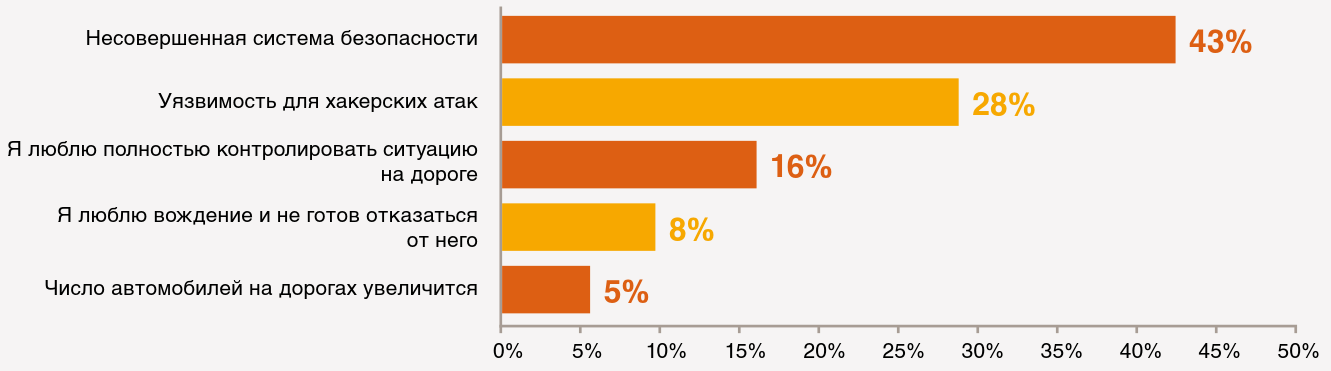
\includegraphics [scale=0.5] {social_disadvantages}
  \caption{Социальный опрос: недостатки автономных транспортных средств}
  \label{img:social_disadvantages}
\end{figure}

7 мая 2016 года автомобиль Tesla Model S, двигавшийся в беспилотном 
режиме, на полном ходу въехал в белую фуру: машина не признала препятствия в 
белом грузовике на фоне белого неба. В результате верхнюю часть автомобиля
полностью снесло (рисунок \ref{img:tesla_crush}), 
а пассажир, один из известных поклонников беспилотных автомобилей, скончался от 
полученных травм \cite{Tesla_Accident}.

\begin{figure}[ht] 
  \centering
  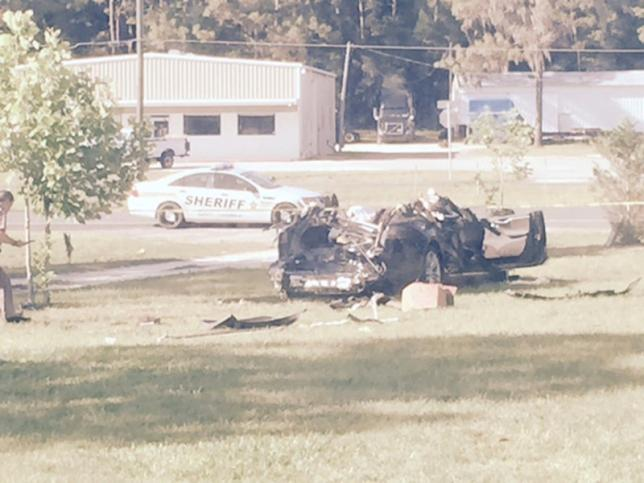
\includegraphics [scale=0.7] {tesla_crush}
  \caption{Tesla Model S после аварии}
  \label{img:tesla_crush}
\end{figure}

Пока беспилотные автомобили еще не готовы к выходу на дороги общего пользования. Они 
неплохо умеют ездить по автобанам, парковаться и заезжать в гараж, но еще слабы 
в перестроениях, обгонах, проездах оживленных перекрестков и прочих простых 
операциях, не говоря уже о нестандартных ситуациях. Технически на то есть две 
основные причины.

Во-первых, ни один из типов современных датчиков (используются 
обычные камеры, инфракрасные камеры, радары, ультразвуковые датчики и лазерные 
дальномеры — лидары) не способен дать машине достаточной информации об 
окружающем мире. Поэтому разработчики вынуждены использовать сразу несколько 
типов сенсоров и составлять единую картину из разнородной информации, что часто 
бывает дорого, долго и сложно.

Во-вторых, современные системы искусственного интеллекта еще не чувствуют 
дорогу так, как чувствует ее человек. Они не всегда понимают, как полоса 
движения может быть свободна только наполовину, не видят подвешенных в воздухе 
препятствий и вряд ли сориентируются на забитом машинами перекрестке, где все 
водители едут уже не по правилам, а ориентируются по одним им понятным и еле 
уловимым движениям глаз и рук.

%%%%%%%% Безопасность %%%%%%%%%
% http://www.tadviser.ru/index.php/%D0%A1%D1%82%D0%B0%D1%82%D1%8C%D1%8F:%D0%90%D0%B2%D1%82%D0%BE%D0%BF%D0%B8%D0%BB%D0%BE%D1%82_(%D0%B1%D0%B5%D1%81%D0%BF%D0%B8%D0%BB%D0%BE%D1%82%D0%BD%D1%8B%D0%B9_%D0%B0%D0%B2%D1%82%D0%BE%D0%BC%D0%BE%D0%B1%D0%B8%D0%BB%D1%8C)#.D0.91.D0.B5.D0.B7.D0.BE.D0.BF.D0.B0.D1.81.D0.BD.D0.BE.D1.81.D1.82.D1.8C
%%%%%%%%%%%%%%%%%%%%%%%%%%%%%%%

В октябре 2017 года, выступая на Всемирном форуме знаний в Сеуле, Южная Корея, 
главный исполнительный директор Mobileye и старший вице-президент Intel, 
профессор Амнон Шашуа предложил автомобильной отрасли способ, 
позволяющий подтвердить безопасность беспилотных автомобилей. Его решение, 
опубликованное в научной статье и представленное в кратком изложении этой 
работы для обывателей, предлагает математическую формулу, используя которую 
можно подтвердить, что тот или иной беспилотный автомобиль работает с 
соблюдением норм ответственности и не может послужить причиной аварии, вину за 
которые можно бы было возложить на этот автомобиль \cite{Intel_Safety}.

Представленная учеными модель Responsibility Sensitive Safety предусматривает 
конкретные, поддающиеся измерению параметры, характеризующие человеческие 
представления об ответственности и осторожности, и определяет так называемое 
<<безопасное состояние>>, поддерживая которое беспилотный автомобиль 
не может послужить причиной аварии, вне зависимости от того, какие маневры или 
действия совершают другие транспортные средства (рисунок \ref{img:intel_safety}).

\begin{figure}[ht] 
  \centering
  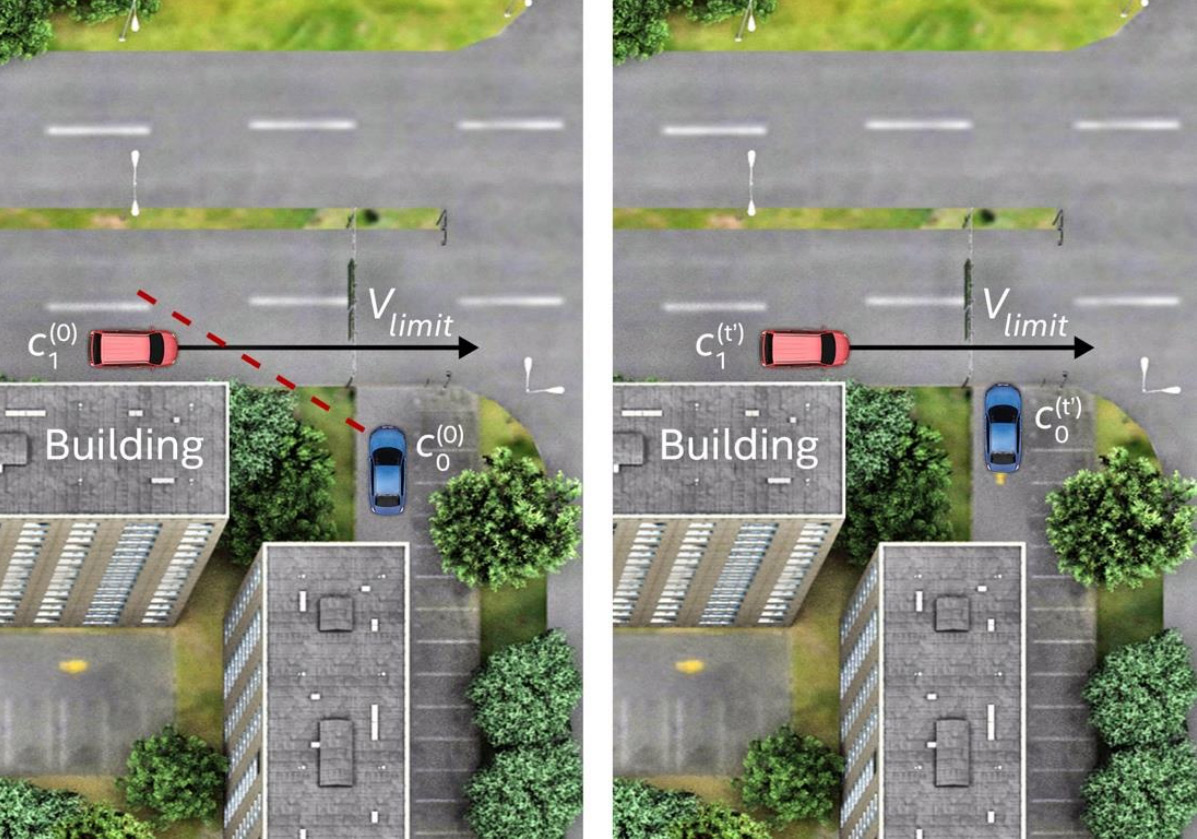
\includegraphics [scale=0.35] {intel_safety}
  \caption{Сценарии для спорных решений беспилотного транспорта}
  \label{img:intel_safety}
\end{figure}

В своем выступлении Амнон Шашуа призвал представителей отрасли и тех, кто 
разрабатывает стратегии, вместе работать над созданием стандартов, которые бы 
позволяли однозначно устанавливать виновника при неизбежных авариях с участием 
автомобилей, управляемых водителями, и беспилотных автомобилей. Все современные 
правила и нормативные акты базируются на той идее, что 
автомобилем управляет водитель, поэтому для регламентирования беспилотных 
автомобилей в правила необходимо вводить новые параметры. 

%%%%%%%% Оптимист %%%%%%%%%
% http://integral-russia.ru/2016/10/10/bespilotnye-avtomobili-bezopasnost-i-budushhee-chast-1/
%%%%%%%%%%%%%%%%%%%%%%%%%%%%

Спорные ситуации на дорогах всегда 
возникали, возникают и будут возникать, и сейчас все они регламентированы как 
раз Правилами дорожного движения (как регламентированы и реальные дилеммы 
вагонеток у машинистов, видящих человека на рельсах, но не имеющих права 
тормозить, чтобы не спровоцировать тяжелых травм у сотен пассажиров). Так, 
при внезапном появлении пешехода на дороге водитель согласно ПДД должен начать 
резко тормозить, но при этом не менять полосы движения, чтобы не спровоцировать 
аварий.

%%%%%%%%%%%%%%%%%%%%%%%%%%%%%%

% Оптимист: «Сейчас про каждую аварию «Теслы» пишут абсолютно все, — говорит 
% руководитель департамента по созданию беспилотных транспортных средств 
% Cognitive Technologies Юрий Минкин. — Это похоже на ситуацию с авиацией на заре 
% ее развития, но теперь мы знаем, что самолет — это самый безопасный транспорт. 
% Точно так же лет через 15—20 и про аварии беспилотников будут говорить уже как 
% про диковинки, трагические стечения обстоятельств, вопиющие нарушения правил».

% Число жертв автомобильных аварий в развитых странах стабильно уменьшается 
% начиная с 1965 года, но, похоже, выходит на свой предел: одна смерть на 100 
% миллионов пройденных километров. Введение подушек безопасности и борьба с 
% алкоголем за рулем сыграли свою роль, но теперь нужно что-то еще — возможно, 
% дело как раз за беспилотниками. Во всяком случае, беспилотные гуглмобили, уже 
% несколько лет проходящие полевые испытания на дорогах Калифорнии, впервые попали 
% в более-менее серьезную аварию с небольшими травмами пассажиров только после 2,7 
% млн километров. С тех пор прошло уже больше года, машины «Гугла» накрутили еще 
% много сотен тысяч километров, а новых аварий больше не было — совсем неплохо для 
% глупой железки.

% Впечатляющих примеров с бепилотниками еще много: в конкурсе Visilab 
% Intercontinental Autonomous Challenge, прошедшем еще в 2010 году, четыре 
% мини-вэна за три месяца проехали почти в автономном режиме 13 тысяч километров 
% от Италии до Китая; в Европе в марте этого года завершился автопробег Euro Truck 
% Platooning, где колонна из 4—5 грузовиков лишь с одним водителем в передней 
% машине одолела более 2 тысяч километров дорог Старого света; наконец, Uber в 
% сентябре этого года и вовсе запустил беспилотное такси на улицах американского 
% Питтсбурга. Правда, во всех этих случаях за рулем беспилотника пока сидели 
% контролирующие их операторы. 


%\newpage
%============================================================================================================================
\section{Проблемы внедрения беспилотного транспорта} \label{sect3_Implementation}

Огромным недостатком беспилотного автомобиля является то, что его использование в
будущем лишит миллионы людей рабочих мест. Создание мобильных сервисов такси такими
известными компаниями как Uber и Яндекс вызвали негатив со стороны таксистов по всему
миру. Так в 2012 году таксисты вышли на митинги против действий сервиса Uber,
блокировали аэропорты и главные улицы, а также требовали от администрации города
прекращения работы этой компании \cite{Plus&Minus}.

В ближайшем будущем беспилотные транспортные средства лишат таксистов рабочих
мест. По некоторым подсчетам, около 4 миллионов водителей станут безработными, и
перевозки станут полностью автоматизированной сферой деятельности.

То же самое ожидает и грузовой транспорт. В 2017 году одна из российских
транспортных компаний заявила, что скоро в Москве начнется активное использование
беспилотные автомобили для доставки грузов \cite{Pilotless_Economics}.

Следующим недостатком является отсутствие законодательной базы по регулированию
беспилотных транспортных средств. Проблема состоит в том, как с юридической точки
зрения определить того, кто будет виноват в случае ДТП. На данный момент в большинстве
стран использование беспилотников запрещено, так как разработка законов о регулировании
такого транспорта находится в ранней стадии. Ситуация по США показана на
рисунке \ref{img:us_laws}. Кроме этого, некоторые автомобили еще
имеют небольшие технические браки и недоработки в силу недостатков конструкции
автомобилей и финансовых затрат. Компания General Motors выявила дефект замка
зажигания, по причине которого неожиданно отключался двигатель. Из-за этого инцидента
пришлось отозвать большое количество автомобилей. Подобные недочеты способны
принести компании большие убытки.

\begin{figure}[ht] 
  \centering
  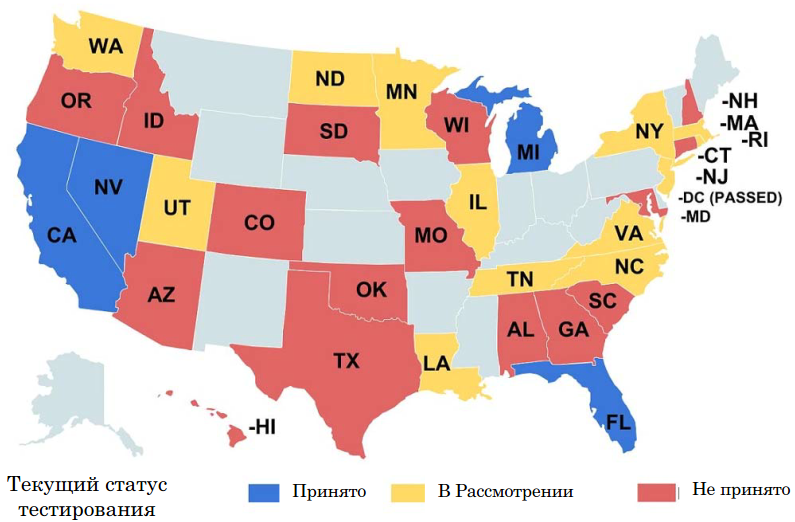
\includegraphics [scale=0.7] {us_laws}
  \caption{Ситуация в разрешением на тестирование автороботов в США}
  \label{img:us_laws}
\end{figure}

Американский законодательный орган может принять закон об освобождении от
ответственности беспилотных автомобилей. Поскольку более 90\% ДТП случаются из-за ошибок
водителей, то использование беспилотных автомобилей должно привести к резкому
снижению травматизма и гибели людей на дорогах. Это приводит к положительному
результату, несмотря на небольшое количество ДТП из-за технических сбоев. Другие
технологические новшества уже демонстрировали подобную статистику. Например,
подушки безопасности спасают больше жизней, чем уносят из-за ошибочного 
срабатывания \cite{Homo_Robo}.
% Начало главы полностью без изменений из Plus&Minus с добавлением рисунков

Высокая цена, обусловленная внутренней технической начинкой машины.
Всевозможные системы автономного управления - это технологическое новшество. Поэтому
цена на такое оборудование на данный момент является заоблачной для обычного
пользователя. Кроме того, многие люди не хотят отдавать крупную сумму за автомобиль,
которым полностью управляет компьютер, так как общество не особо доверяет новой
технике.

Последние разработки в сфере автомобильной индустрии показывают, что прогресс не
стоит на месте. Первые автомобили, заменившие лошадиные повозки, вызывали у людей
настороженность и недоумение. А сейчас таким транспортным средством никого не
удивишь. Однозначно беспилотный автомобиль станет новой ступенью в развитии
автомобильного транспорта, ведь его появление всего лишь вопрос времени.
